
\section{Planned Statistical Analysis}
\label{ch:analysis}
The analysis asks whether the two voice configurations differ in efficiency and experience. Active completion time is the primary outcome, workload and motivation are secondary, and agent experience, reliance, and debrief responses are exploratory. Because each participant experiences both voices, these outcomes are compared within participants, while guidance diagnostics describe exposure and technical context. Jev and gaze contingency are shared by both conditions, so the statistical comparison concerns voice configuration rather than the independent value of those components.

\subsection{Primary Contrast}
The primary estimand compares active completion time under the self-similar and neutral voices, standardized to the same starting-difficulty distribution. A trial-level mixed-effects analysis of log completion time accounts for participant clustering, voice condition, period/order, trial progression and absolute pre-cue starting theta. The analysis reports the voice time ratio and uncertainty using a two-sided contrast.

Nonlinearity in starting difficulty is represented by a prespecified low-complexity function of theta, while nominal-angle strata support balance plots and a categorical sensitivity analysis. Zero-degree trials remain in the analysis, and completion time is not divided by angle. Before confirmatory recruitment, simulation is used to finalize the model's random-effects structure, angle function and smallest meaningful effect. The participant count requires justification under that same model rather than by treating repeated trials as independent participants.

Figure~\ref{fig:analysis-units} illustrates the planned units of observation. Trial-level measurements are nested within participants, while retrospective ratings remain participant-by-block observations.

\begin{figure}[htbp]
\centering
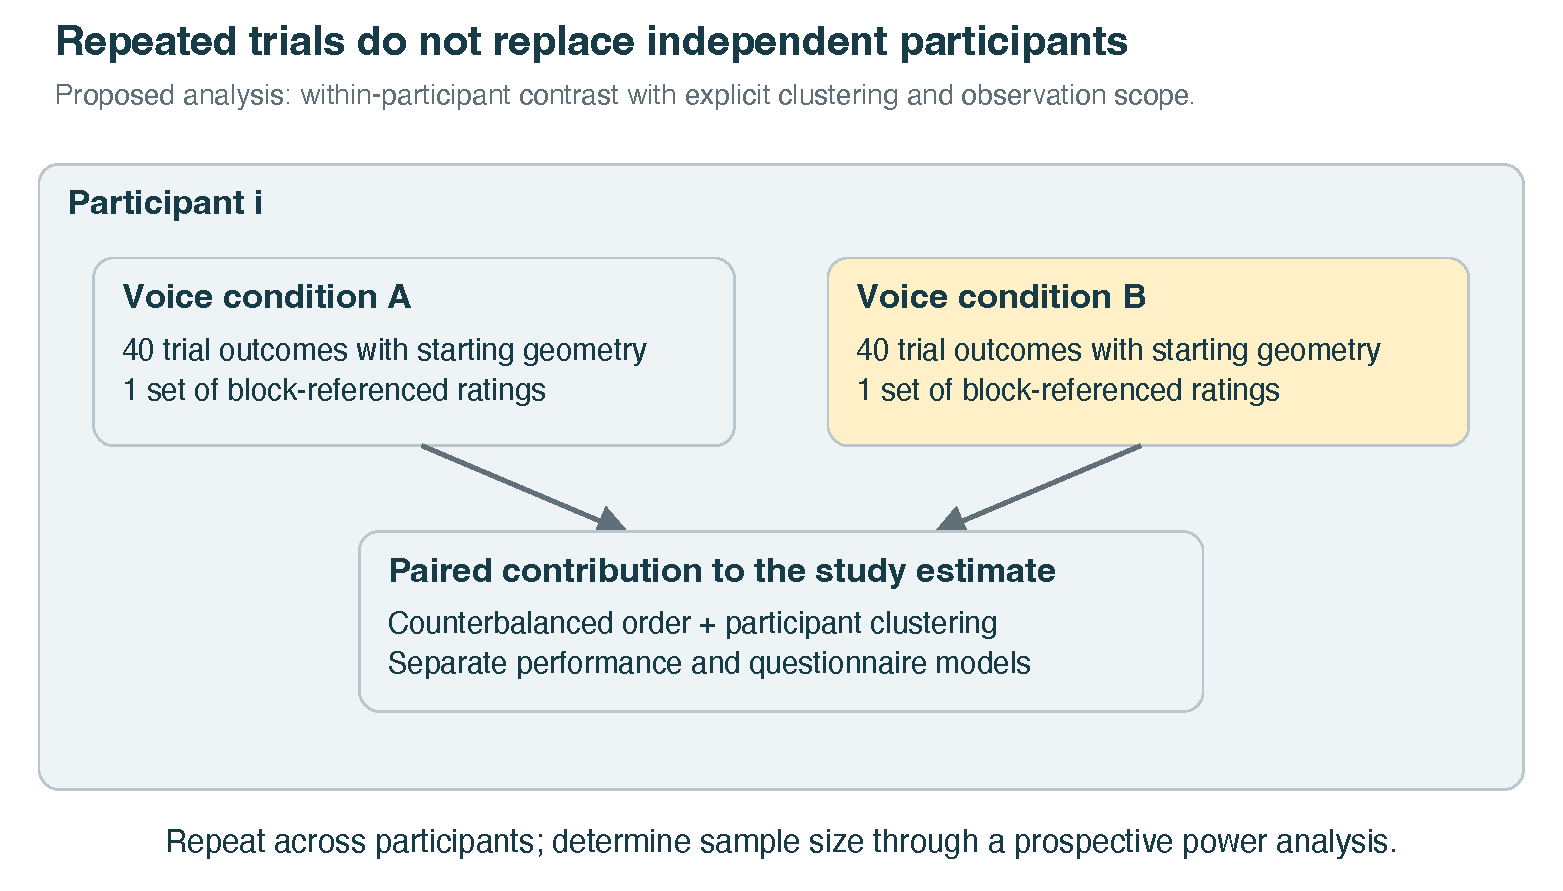
\includegraphics[width=\linewidth,alt={Participant contains two voice conditions, each with 40 trial outcomes and one retrospective questionnaire set, feeding a paired study contrast.}]{figures/analysis-units.pdf}
\caption[Trial nesting and questionnaire analysis units]{Proposed analysis scope. Each participant contributes repeated trial outcomes and two block-referenced questionnaire sets. Counterbalanced order and participant clustering remain part of the analysis plan; additional trials do not replace a justified participant sample size.}
\label{fig:analysis-units}
\end{figure}

Table~\ref{tab:analysis-scope} summarizes the proposed outcome hierarchy and units of analysis. Final contrasts, missing-data handling, and multiplicity families remain to be specified in the preregistration.
\begin{table}[htbp]
\centering
\caption[Planned outcomes and analysis units]{Outcome hierarchy and observation scope. Engineering metrics diagnose the guidance system and do not replace participant outcomes.}
\label{tab:analysis-scope}
\small
\tagpdfsetup{table/header-rows={1}}
\begin{tabularx}{\linewidth}{@{}p{0.20\linewidth}p{0.25\linewidth}X@{}}
\toprule
Role & Unit & Planned interpretation \\\midrule
Primary performance & Trial within participant & Voice contrast in active time, adjusted for starting geometry and design factors. \\
Secondary experience & Participant by referenced block & Workload and separate IMI subscales, retaining paired scope. \\
Exploratory perception & Participant by referenced block & Agent constructs, individual custom items, and voice-similarity manipulation check. \\
Safety & Participant over full session & Recorded discomfort reports, pauses, stops and incomplete exposure. \\
Engineering quality & Qualified event episode / request & Delivery delays, errors, repetition, and provider reliability with distinct denominators. \\
Qualitative experience & Participant response / coded excerpt & Debrief themes with an audit trail, not causal performance estimates. \\\bottomrule
\end{tabularx}
\end{table}

\subsection{A Candidate Primary Model}
A candidate model makes the intended estimand explicit while leaving the final specification to preregistration. For participant $i$, period $b$, and trial $j$, let $Y_{ibj}=\log T_{ibj}$ for successfully completed active-search intervals. A starting specification is
\begin{align}
Y_{ibj}={}&\beta_0+\beta_V V_{ib}+\beta_B B_b+\beta_O O_i\\
&+f(|\theta_{0,ibj}|)+g(j)+u_{0i}+u_{Vi}V_{ib}+\epsilon_{ibj}.
\end{align}
Here $V$ indicates self-similar rather than neutral voice, $B$ identifies the second period, and $O$ identifies assigned voice order. The functions $f$ and $g$ represent prespecified low-complexity effects of exact starting angle and trial progression. In this candidate specification, $j$ indexes position within a block (1--40); the period term represents the between-block change. The exact pre-cue angle depends on the snapshot described in Section~\ref{ch:measurement}, which has not yet been implemented; until it is, the model cannot be fitted as specified, and nominal wall angles must not be relabeled as exact measurements to fill that gap. Participant intercepts and, if supported by the design and model stability, participant voice slopes represent clustering and variation in within-participant contrasts. With only one block per voice, the slope variation can also absorb block-specific session effects; it is not a pure measure of stable individual voice responsiveness. The final random-effects structure remains open; its selection depends on the experimental design and simulation rather than statistical significance~\cite{barr2013random}.

Under this model, the exponentiated voice coefficient, $\exp(\beta_V)$, is a conditional multiplicative time contrast and does not automatically equal a marginal arithmetic mean ratio. The primary estimand therefore remains the marginal contrast standardized over the prespecified common starting-difficulty distribution; the conditional coefficient is reported separately as a model parameter rather than substituted for that estimand. Predictions on the original seconds scale require an explicit retransformation procedure and uncertainty estimate.

A two-period design supports adjustment for period and sequence, but cannot identify every possible asymmetric carryover mechanism independently. For example, using a voice during practice could affect familiarity in its first block, and the second block could benefit from task learning. Period and order terms therefore address these influences only partially, and the report describes residual carryover as a limitation.

\subsection{Sample Size and Precision Planning}
Forty trials per block increase the information available within each participant, but one participant's 80 trials remain correlated observations rather than a substitute for additional participants. A power analysis must reflect the planned trial-level model, between-participant heterogeneity, within-participant correlation, geometry distribution, incomplete trials, and the effect size worth detecting.

The proposed simulation workflow generates participants with both voice blocks and the intended nominal-angle quotas, varying plausible residual variation, participant intercept variation, voice-slope variation, and missingness. Each simulated dataset is fitted with the same model intended for the final analysis, and convergence, bias, interval coverage, and power or precision are summarized across candidate enrollment sizes. The chosen smallest meaningful time ratio and its supporting assumptions require documentation before recruitment. Synthetic pilot values used to test the workflow are labeled as such and are not presented as empirical variance estimates.

A retained pilot can inform variance assumptions only under a documented rule about whether those observations enter the confirmatory sample. The study preserves a build and protocol identifier so that a pilot collected under a different guidance policy can be separated from the frozen release.

\subsection{Secondary Outcomes and Multiplicity}
Condition-specific ratings are collected retrospectively, only after both blocks, with actual survey timestamps retained; each rating set nevertheless remains referenced to a participant-by-block observation. Because these are not immediate post-block measurements, recall and recency effects are considered when interpreting condition differences. Individual workload dimensions and complete unweighted workload means are summarized by participant and block. IMI subscales and the three six-item agent-perception constructs remain separate scores, and the additional Guo Q20--22 appealing, eerie and familiar ratings are analyzed individually rather than combined into an eeriness score. Voice similarity serves as a manipulation check, while custom experience ratings and self-reported guidance use are also analyzed individually.

The analysis retains paired observations and accounts for period where appropriate. The choice between ordinal-item and approximately continuous scale models requires a justification for each measure before confirmatory analysis.

Multiplicity families, secondary contrasts, and adjustment rules require specification before confirmatory analysis. Holm's procedure is available for a prespecified family of confirmatory secondary comparisons~\cite{holm1979simple}; it is not a substitute for deciding which outcomes belong in that family. Exploratory agent-perception and custom-item results are labeled, with effect estimates and uncertainty rather than an indiscriminate list of significance claims.

A participant who does not recognize the clone provides information about the strength of the manipulation and is not excluded solely on that basis; similarly, low liking of either voice is an outcome rather than grounds for exclusion. Sensitivity analyses may examine synthesis quality or recognition, but conditioning on experience that follows assignment changes the interpretation of the contrast, and that change is stated.

\subsection{Data Screening and Missingness}
Data screening first establishes structural integrity: unique participant/session/block/trial keys, consistent voice assignments, chronological reveal and selection events, and required geometry provenance. It then assesses observation coverage and protocol deviations.

A trial with sparse gaze coverage may have valid selection timing yet unreliable gaze-contact latency, so exclusion should be measure-specific where justified. A missing gaze contact does not automatically invalidate completion time, and a complete motion stream does not repair missing voice playback events. Each analysis reports its own denominator and reasons for missingness.

Stopping, timeout, withdrawal, and technical failure require a prespecified treatment. A complete-case time model estimates completion times among observed successful trials under its assumptions, and it may not describe all assigned trials if incomplete outcomes differ by voice. The final plan must therefore also define a complementary completion-probability or time-to-event analysis for use if incompletion is consequential. The revised protocol fixes the active-search deadline at 25 seconds. Deadline-expired attempts are unsuccessful outcomes for completion probability and right-censored at 25 active seconds for a time-to-event analysis; they are not successful 25-second completion times. Earlier development recordings predate this rule and retain their original exposure.

Raw attempts, incorrect selections, pause intervals, timeouts, technical failures and withdrawals are all retained, and stopped trials are not coded as successful completion times. The deadline outcome is recorded separately from technical failure and withdrawal. The remaining treatment of those interruptions and the missing-data estimand require specification before collection; slow successful trials within the deadline are not removed solely for being slow. Missing responses are not replaced with zero; questionnaire scores follow the complete-subscale rule, with item-level missingness reported.

\subsection{Behavior as Outcome Rather Than Automatic Adjustment}
Instruction count, gaze path, and controller behavior can be consequences of voice condition. Including them automatically as primary-model covariates could remove part of the effect the study intends to estimate. The primary comparison therefore adjusts for pre-cue difficulty and design variables. Voice-by-theta variation, selected neutral voice, acoustic quality, guidance timing, and search behavior enter exploratory or sensitivity analyses with their assumptions reported.

For example, slower search can produce more opportunities for guidance, and more guidance can itself affect search time. A correlation between instruction count and duration does not establish that speech caused delay.

\subsection{Guidance Delivery Evaluation}
Engineering analysis distinguishes event qualification, decision latency, model deferral, scheduling delay and actual playback, and it evaluates gaze and controller confirmation separately. Sequence-level review includes what happened before and after each cue. Automatic checks and ratings produced by an offline language-model evaluator (Appendix~\ref{app:scenarios}) remain advisory engineering evidence rather than participant perception scores.

\subsection{Additional Performance and Eye-Behavior Figures}
Missed-target percentages complement completion-time distributions, with the number of completed, timed-out, technically interrupted, and unresolved attempts shown explicitly. For the participant study, paired participant summaries by voice condition are preferable to treating all trial rows as independent observations. Earlier unconstrained development recordings are kept separate from searches governed by the new deadline.

After independent detector validation, possible additional figures include fixation-count distributions, saccade rates with their valid-time denominators, and IPA distributions with retained pupil coverage, each separated by voice condition and participant. Last-target-fixation duration requires validated events and a target-area join. No EEG or ERP plot can be generated from the current headset logs. Until those requirements are met, the candidate-eye figures in Section~\ref{sec:development-eye-candidates} serve only to inspect the processing pipeline; they do not test a voice effect or infer workload. Threshold sensitivity and missing-data summaries accompany each derived outcome.

\subsection{Qualitative Analysis and Mixed Evidence}
The debrief begins with broad experience questions, followed by balanced probes about voice preference, perceived performance, comfort, and potential uses. The coding process records the initial codebook, revisions, coding decisions, and independent review of a subset. Contradictory or minority accounts are retained rather than forced into one favorable theme.

Reported reliance and observed behavior are considered together without treating either as a perfect measure of the other. The final report separates quotations, coder interpretation, and behavioral evidence.

\subsection{Safety Outcomes and Manipulation Checks}
Safety reporting describes recorded discomfort reports, pauses, stops and incomplete exposure, including the reason for each interruption when available. These observations document tolerability and session completion; they do not provide a standardized pre-to-post symptom score. The operational stopping procedure must be frozen before participant collection.

The similarity manipulation check reports the paired difference between self-similar and neutral-voice ratings with uncertainty. A group-level decision rule and any practically meaningful difference remain open preregistration decisions. Because equivalence testing is not currently specified, a nonsignificant voice contrast is not interpreted as equivalence.
